\section{Theory}
The band gap of a material is the minimum difference in energy between the highest energy state of the valence band and the lowest energy state of the conduction band. Determination of the band gap of a semiconductor is one of the important and basic thing in solid state physics as it provides critical information for understanding the band structure of material.

\begin{figure}[h]
    \centering
    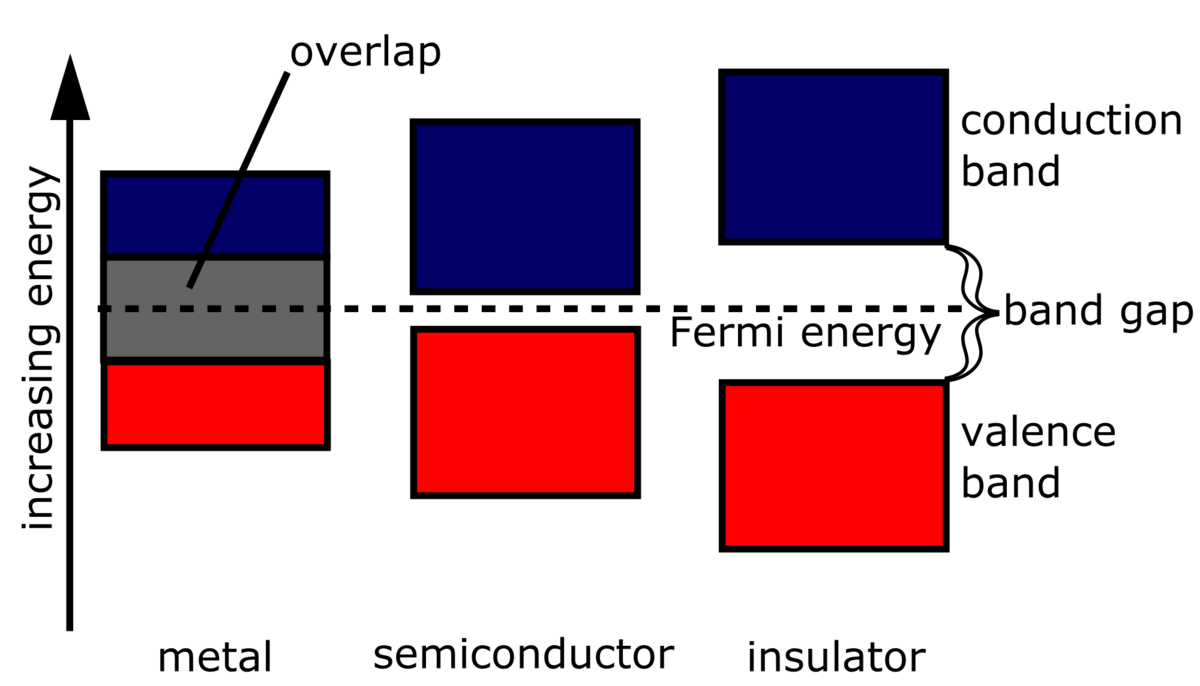
\includegraphics[width=1\columnwidth]{images/th1.png}
    \caption{Illustration depicting the conduction and valence bands along with the corresponding bandgaps for different types of materials}
    \label{f1}
\end{figure}

There are several well accepted ways to determine the bandgap of semiconductors including the four-probe method, UV-spectroscopy, by the temperature variation of resistivity or forward voltage (keeping the forward current constant) etc. In this experiment, we have presented a way to determine the band-gap of semiconductors by the studying the temperature variation of reverse current in the diode, following up on \citeauthor{biswas-2022} (\citeyear{biswas-2022}). 

\subsection{Mathematical Formulation}
When a pn junction diode is operated under reverse bias conditions, a very small amount of current flows through the diode, called the \textit{reverse current}. The magnitude of this current is almost negligible ($\sim\,\mu$A) and is generated due to the thermally generated minority charge carriers on each side of the junction. 

\begin{figure}[h]
    \centering
    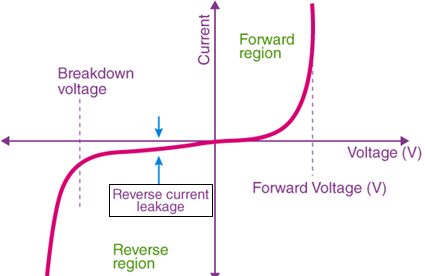
\includegraphics[width=1\columnwidth]{images/th2.png}
    \caption{Typical I-V characterstic of a pn junction. The reverse current is highlighted and is quite negligible under normal conditions.}
    \label{f2}
\end{figure}

For a fixed reverse bias potential, the number of minority charge carriers generated thermally now purely depends on the temperature of the system. 

Mathematically, we can write the reverse current $I_r$ as,
\begin{align}
    I_r = A \exp({-\frac{E_g}{\eta k_B T}})
\end{align}
\noindent where $A$ is a constant, $E_g$ is the band-gap of the material used, $k_B$ is the Boltzmann constant, $T$ is the temperature and $\eta$ is the diode quality factor. Typically $\eta=1$ for Ge and for Si, $\eta=2$.

Now, taking log on both sides of the above equation,
\begin{align}
    \ln{(I_r)} = \ln(A) - \frac{E_g}{\eta k_B T}
\end{align}

It is to be noted that $E_g$ itself is a function of temperature (\citeauthor{varshni-1967}, \citeyear{varshni-1967}),
\begin{align}\label{temp}
    E_g = E_0 - \frac{\alpha T^2}{\beta + T}
\end{align}
\noindent i.e., $E_g$ decreases with increase in temperature where $E_0$ denotes the band gap at absolute zero temperature and $\alpha$ and $\beta$ are two constants. The major reason for this is the shift in the relative position of the conduction and valence bands due to a temperature-dependant electron lattice interaction. Experimentally we have determined, $\alpha \sim 10^{-4}$ and $\beta \sim 10^3$. Due to this, fractional term is quite small compared to $E_0$ for the temperature range used in this experiment, we can assume $E_g \approx E_0$.

Thus, Eq. 2 simplifies to 
\begin{align}\label{eq4}
    \ln{(I_r)} \approx \ln(A) - \frac{E_0}{\eta k_B T}
\end{align}

Now, if we measure the value of $I_r$ at different temperatures, we can find determine $E_0$ from the slope of the straight-line fit of a $\ln(I_r)$ vs $T^{-1}$ plot. That is, Eq. \ref{eq4} is of the form,

\begin{align}
    y = mx + c
\end{align}

where $y=\ln(I_r)$, $x=1/T$ and 
\begin{align} \label{slope}
    m = -\frac{E_0}{\eta k_B}\\
    c = \ln(A)
\end{align}
% ===================================================================
\section{Experimental Setup}

\subsection{Apparatus}

\begin{enumerate}
    \item ExpEYES-17 kit + Computer
    \item Germanium Diode (1N60)
    \item Resistors (one 1 k$\Omega$ and two 100 $\Omega$)
    \item Soldering iron
    \item Chromel/Alumel Thermocouple for temperature measurement
    \item Wooden Board to fix the setup
\end{enumerate}

\subsection{Circuit Design}

\begin{figure}
    \centering
    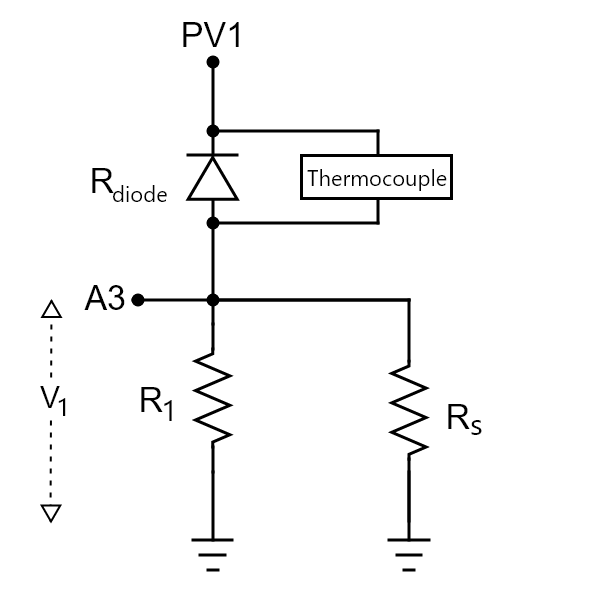
\includegraphics[width=.8\columnwidth]{images/circuit.png}
    \caption{Circuit diagram with connections to terminals of the SeeLab module}
    \label{c1}
\end{figure}

\begin{figure*}
    \centering
    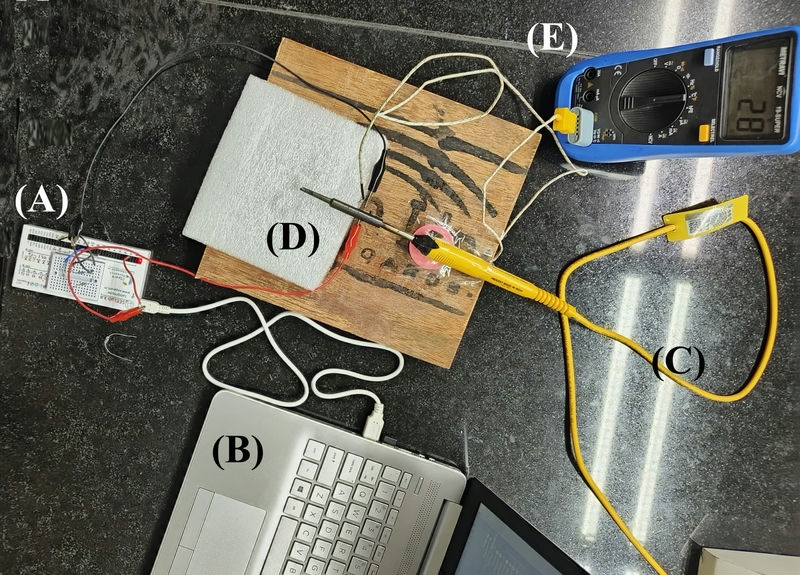
\includegraphics[width=1.3\columnwidth]{images/pic.jpg}
    \caption{Experimental setup where (A) is the SeeLab module connected as per the circuit diagram to the (B) computer. (C) is the soldering iron attached to a wooden board (D) on which the diode is also attached. (E) is the multimeter connected to the thermocouple which reads the temperature of the diode.}
    \label{c2}
\end{figure*}

The circuit diagram of the setup is shown in Fig. \ref{c1}. $R_s$ is the shunt resistance connected across $R_1$ to measure the voltage across the diode. If $V_1$ is the measured voltage across $R_1$ by terminal \verb|A3|, then the reverse current through the diode is given by,

\begin{align} \label{ir}
    I_r R_1 &= \frac{V_1 R_s}{R_s + R_\text{diode}} \nonumber\\
    \implies I_r &= \frac{V_1}{GR_1}\\\text{ where, } G &= 1+ \frac{R_\text{diode}}{R_s} \nonumber
\end{align}

\subsection{Procedure}
The experimental setup and circuit diagrams are shown in Figs. \ref{c1} and \ref{c2}. The procedure of the experiment is detailed below.\\

\begin{enumerate}
    \item Begin by fixing the soldering iron on a wooden board and attach the diode near it so that it is not in direct contact.
    \item Attach the thermocouple as close as possible to the diode to measure accurate temperature readings.
    \item Connect the diode to the SeeLab breadboard setup and make connections according to the given circuit diagram. Connect the board to the computer and provide around 4V reverse bias voltage to \verb|PV1| using following Python code:
    \begin{lstlisting}[language=Python]
import eyes17.eyes
board = eyes17.eyes.open()
board.set_pv1(4)
\end{lstlisting}        
    \item Now read the voltage values at \verb|A3| using  
    \begin{lstlisting}[language=Python]
v1 = board.get_voltage('A3')
\end{lstlisting}  
\item Also note the corresponding temprature reading on the thermo-couple.
    \item Calculate $I_r$ from $V_1$ using Eq. \ref{ir}.
    \item Plot $\ln(I_r)$ vs. $\ln(T)$ and estimate $E_0$.
\end{enumerate}